% !TeX root = ../main.tex
%
\chapter{Implementation}
To implement the control designs discussed here in \textit{Part 1} it is necessary to estimate some parameters, compensate for any friction between the cart and the rail and filter the measurements obtained from the system. Such considerations, estimations and designs are discussed in this section.

\section{Cart Friction and Mass Estimation}
The control designs are carried out under the assumption that there is no friction between the cart and the rail. It turns out that this friction is rather complex and also depend on position and direction of the cart in addition to its velocity, this issue was also found by previous project groups \cite{JHHorgensen}.\\
To accommodate the no cart friction assumption, a feed forward friction compensator is designed. The idea is to simply counter the predicted friction at any given time directly in the control signal.

Since the friction depends on the cart position, the estimation must be done locally for each position on the rail. To do so, the pendulum masses are removed, the rods strapped to the cart to limit dynamics and the cart is made to oscillate around each centimeter of the rail. Each test is sustained for \SI{20}{s} and repeated for each centimeter, resulting in a total of 68 tests. This is the largest possible range for the test while avoiding impact at the ends of the rail. Each test spans on average \SI{2.68}{cm} creating some overlap between tests. The reduced dynamics used for the estimation are given by,
\begin{align}
  ( M + m )\ddot{x} &=  u - b_{c,v} \dot{x} - \tanh(\text{k}_\text{tanh}\dot{x}) b_{c,c} \ \ \ .
  \label{eq:reducedForCartEstimation}
\end{align}
%
The optimization fitting tool, Senstools \cite{MHKnudsen}, is used to estimate the model parameters. Since the mass is unknown it is also included for estimation. The mass is estimated to be \SI{6.28}{kg}. With more parameters more manual tuning is required in order to start close enough for the optimization algorithm to converge. To reduce the number of parameters as much as possible, once estimated, the mass is fixed as part of the model. The remaining three parameters are viscous friction and coulomb friction for negative and positive velocities. After some trail and error it is concluded that the viscous friction is negligible compared to the coulomb frictions finally leaving only two parameters.\\
To make the estimations converge without too much manual tuning only part of each test is fitted, see \autoref{fig:manyEst}. The time window is moved, and the estimation is run again. The window is moved \num{34} times resulting in $34\cdot68 = 2312$ estimations in total. Every time the test window is moved, the next estimate is started with the results of the previous estimate as its initial values.
%
\begin{figure}[H]
  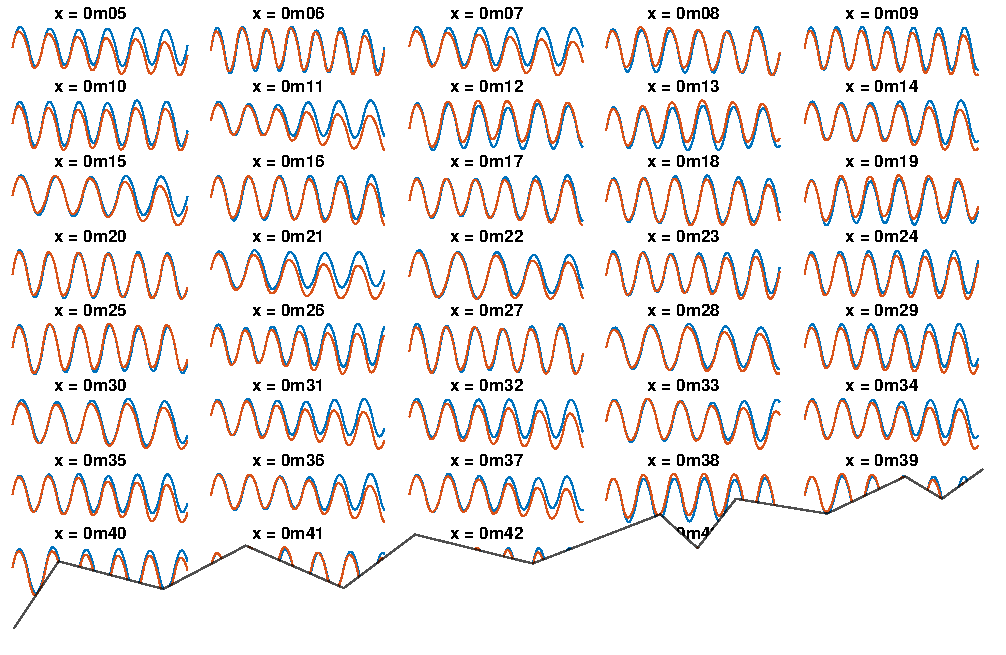
\includegraphics[width=.6\textwidth]{figures/manyEst_tear}
  \caption{A snippet of the estimation of cart Coulomb friction. Each title shows where on the rail the test is done. This is one iteration of 34 moving over the \SI{20}{s} tests.}
  \label{fig:manyEst}
\end{figure}
%
To include as much data as possible, the estimate is repeated across the data for each test, resulting in \num{34} results for each position. The error norm is saved for all estimations, see \autoref{fig:cartErrn}, and a weighed average using the error norm as weights is made for each position on the rail resulting in \autoref{fig:cartColoumb}.
%
\begin{figure}[H]
  \hspace{1cm}
  \captionbox
  {
    Results of the estimations, where the scattered points are all estimates and the lines are the weighed averages using the error norm of each estimate as weights.
    \label{fig:cartColoumb}
  }
  {
    \hspace{-1cm}
    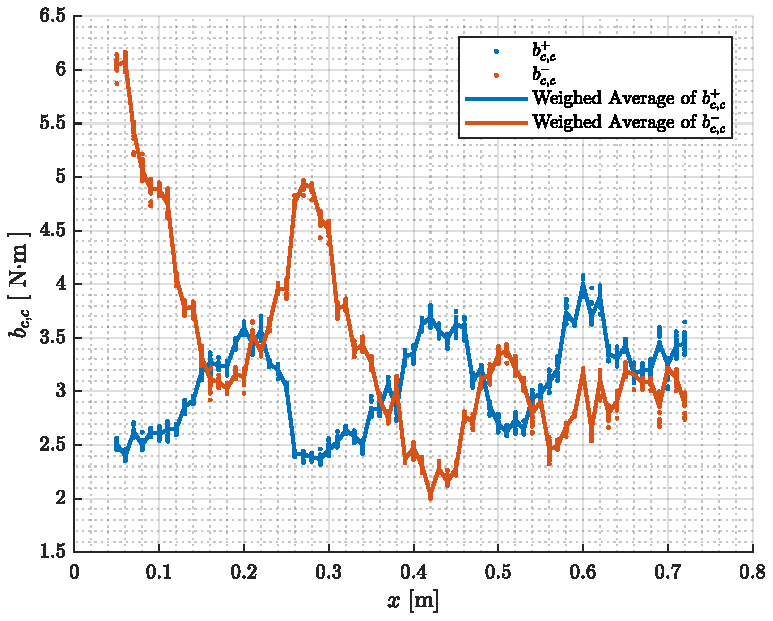
\includegraphics[width=.45\textwidth]{figures/cartColoumb}
  }
  \hspace{20pt}
  \captionbox 
  {
    This shows the error norms for all estimates. There is a clear tendency to worse fits at the left end of the rail. The reason is unknown.
    \label{fig:cartErrn}
  }
  {
    \hspace{-1cm}
    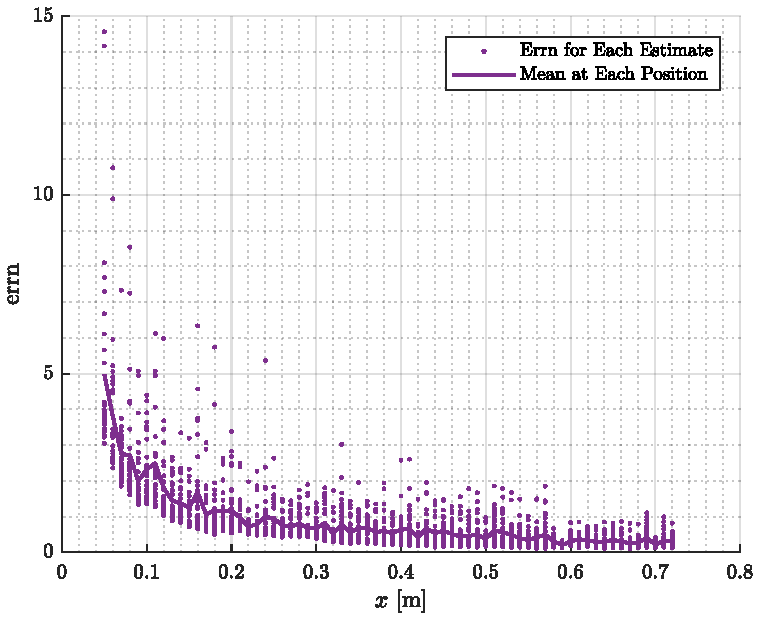
\includegraphics[width=.45\textwidth]{figures/cartErrn}
  }  
\end{figure}
%
The estimations are worse near the left of the rail, see \autoref{fig:cartErrn}. The cause for this is not known, however it is considered less important as the compensation is more critical near the middle of the rail where the pendulum is balanced.

The result in \autoref{fig:cartColoumb} contains some undesired discontinuities. To solve this problem the resulting mean curves are up-sampled by linear interpolation, smoothed and finally down-sampled to obtain the smoothed result in \autoref{fig:cartColoumbSmoothDownSample}.
\begin{figure}[H]
  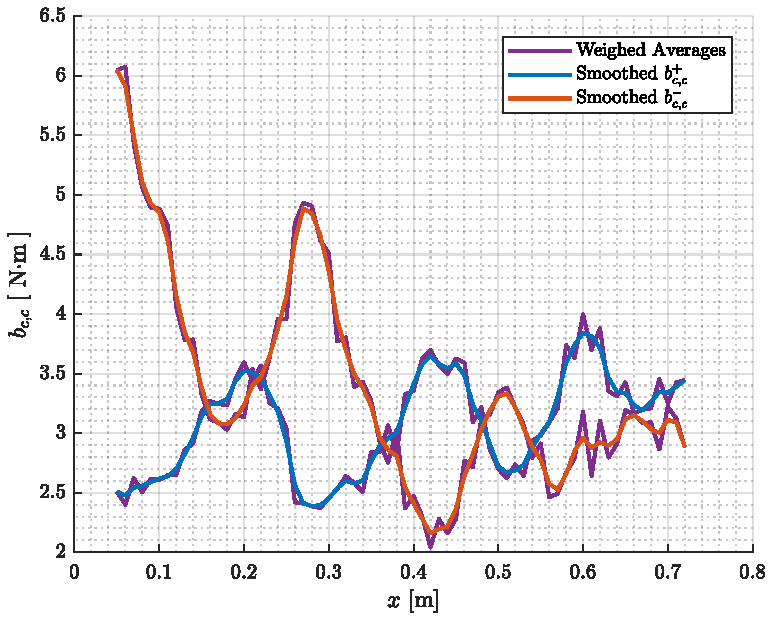
\includegraphics[width=.42\textwidth]{figures/cartColoumbSmoothDownSample}
  \caption{This is the final result of the estimation, which is up-sampled, smoothed and finally down-sampled to produce the values for implementation in lookup-table.}
  \label{fig:cartColoumbSmoothDownSample}
\end{figure}
The result is implemented as lookup tables along with a linear interpolation function to avoid discontinuities between table entries. This determines the cart Coulomb friction based on velocity, direction and position, which is then added to the control signal to counter the friction therm in the dynamics.

\section{Pendulum Friction}
With the cart mass estimated and its friction handled by friction compensation, the remaining estimate is pendulum friction. Again Senstools is used along with a reduced model of the pendulum,
%
\begin{align}
  m l ^2 \ddot{\theta} &= m g l  \sin \theta - b_{p,v} \dot{\theta} - \tanh(k_{tanh} \dot{\theta}) b_{p,c} \ \ \ .
  \label{eq:reducedForPendulum1Estimation}
\end{align}
%
This model assumes there is no cart, so for the test, the cart is fixed to the rail. The result of the test and estimation is seen in \autoref{fig:pendulum1Est}.
%
\begin{figure}[H]
  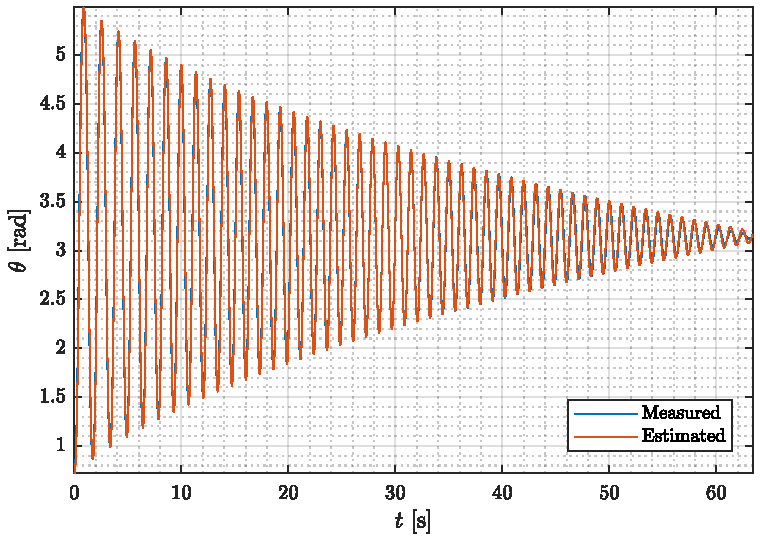
\includegraphics[width=.7\textwidth]{figures/pendulum1Est}
  \caption{The fit resulting in the estimations of the pendulum friction.}
  \label{fig:pendulum1Est}
\end{figure}
%
To obtain a good fit, \SI{22.5}{g} is added to the measured mass and \SI{0.66}{cm} is subtracted from the measured length of the rod. This is presumed to be reasonable, since the rod is otherwise assumed to be massless which is not the case. The error in the assumption would move the mass center closer to the pivot point, thus reducing the effective length of the rod and adding some mass to the weight, corresponding to the adjustments. The pendulum Coulomb friction, $b_{p,c}$, is estimated to \SI{4.1e-3}{N\cdot m} and the viscous friction, $b_{p,v}$, to \SI{0.5e-3}{N\cdot m\cdot s}.

\section{MA Filter Design}
The measurements in the system are the position, $x$, of the cart and the angle, $\theta$, of the pendulum. Thus, the last two states, $\dot{x}$ and $\dot{\theta}$, must be estimated for the implementation. To that end, a numerical differentiation is applied to the position measurements in order to obtain the velocities,
\begin{align}
  \dot{x} &= \frac{x_0 - x_{-1}}{T_{s}}   \ \ \ ,
  \label{eq:nummericalDiff}
\end{align}
where $T_s$ is the sample time and $x_0$ and $x_{-1}$ are the two latest samples. However, this approach causes noise in the velocities. Thus, an MA (Moving Average) filter is designed to smooth the signal,
%
\begin{align}
  \dot{x}_{est} &= \frac{1}{N}\sum_{i=1-N}^{0} \dot{x}_i   \ \ \ ,
  \label{eq:MA}
\end{align}
%
where $\dot{x}_0$ is the numerical differentiation based on the two latest measurements, $x_{est}$ is the filtered value and $N$ is the window size of the filter. In \autoref{fig:thetaDotMA_design} and \ref{fig:xDotMA_design} the MA filter is applied to the result of the numerical differentiation with two different window sizes. Since the interest here is quality of the signal, the following plots are not linked in time, but rather showing the signals where the filter characteristics shows clearly.
%
\begin{figure}[H]
  \hspace{1cm}
  \captionbox
  {
    The result of applying the MA filter to the numerical differentiation of $\theta$ with two window sizes. For $N = 5$ a lot of noise is still in the signal, however, though $N=15$ removes more noise it also introduces unwanted delay. 
    \label{fig:thetaDotMA_design}
  }
  {
    \hspace{-1cm}
    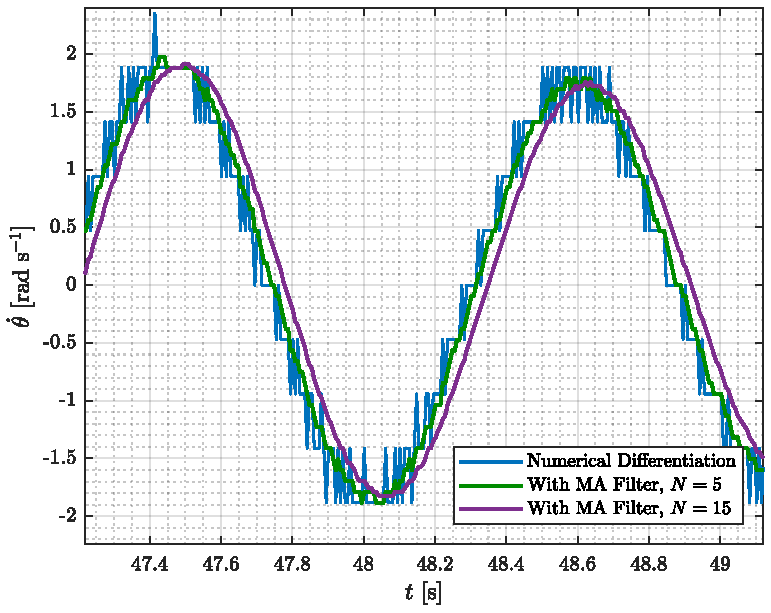
\includegraphics[width=.45\textwidth]{figures/thetaDotMA_design}
  }
  \hspace{20pt}
  \captionbox 
  {
    For $\dot{x}$ the same result is observed, but since the signal is smaller relative to the noise, it more clearly shows the noise issue of the small window size.
    \label{fig:xDotMA_design}
  }
  {
    \hspace{-1cm}
    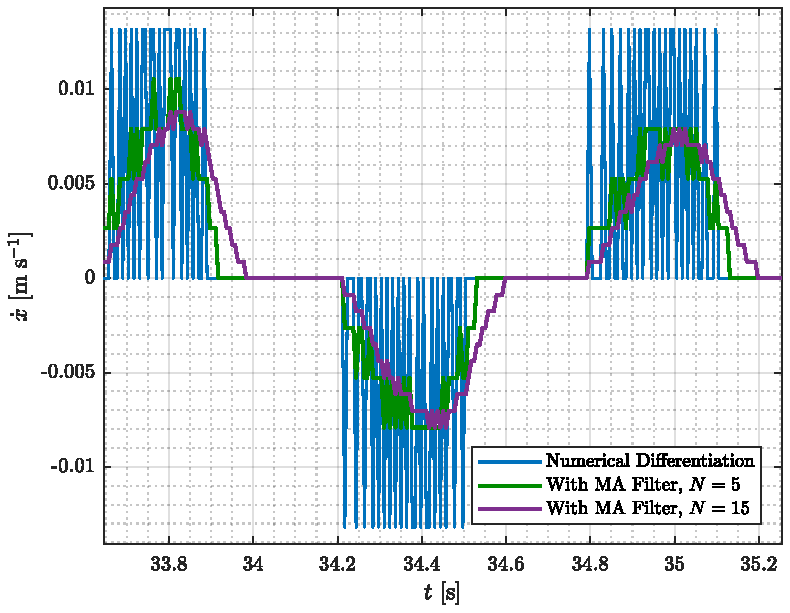
\includegraphics[width=.45\textwidth]{figures/xDotMA_design}
  }  
\end{figure}
%
The filter is implemented using a ring-buffer to minimize computation time and different window sizes are tested. Minimizing delay of the filter turns out to be more critical than further noise reduction, so a window size of five is chosen. The result of the implemented MA filter is shown in \autoref{fig:thetaDotMA_test} and \ref{fig:xDotMA_test}.
%
\begin{figure}[H]
  \hspace{1cm}
  \captionbox
  {
    The resulting implementation of the MA filter with $N=5$ for estimation of $\dot{\theta}$.
    \label{fig:thetaDotMA_test}
  }
  {
    \hspace{-1cm}
    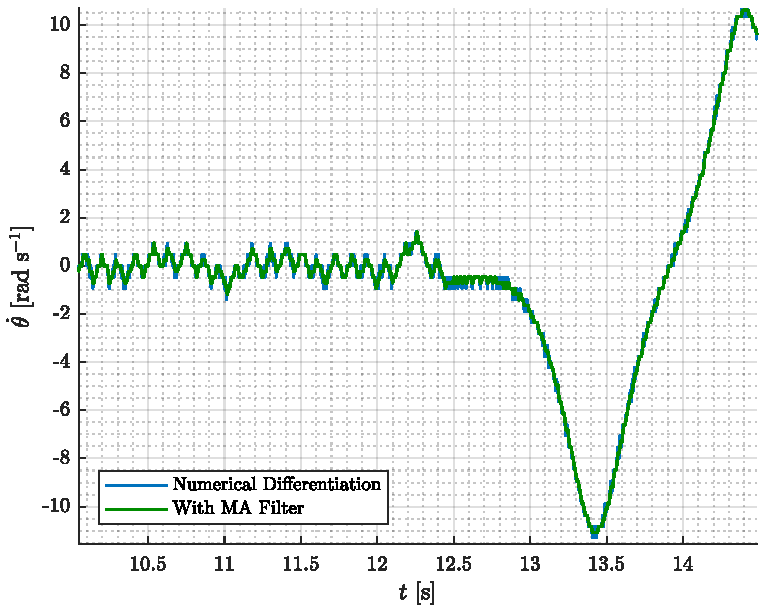
\includegraphics[width=.45\textwidth]{figures/thetaDotMA_test}
  }
  \hspace{20pt}
  \captionbox 
  {
    The implemented MA filter with $N=5$ for estimation of $\dot{x}$.
    \label{fig:xDotMA_test}
  }
  {
    \hspace{-1cm}
    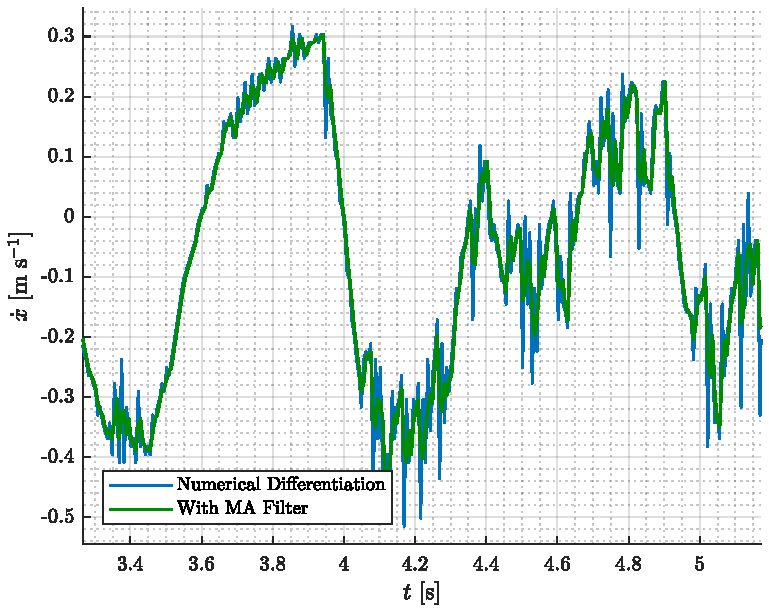
\includegraphics[width=.45\textwidth]{figures/xDotMA_test}
  }  
\end{figure}
%
Though the MA filter still lets a lot of noise through, the design does suppress large jumps in the velocity with very minimal delay.\\
This filter is only used in the swing-up sequence, an extended Kalman filter (EKF) implemented by a previous project group, \cite{JHHorgensen}, is used for the catch sequence as the switching nature of a sliding mode controller would cause oscillations with high noise levels around zero.